\chapter{“MCTrack: A Unified 3D Multi-Object Tracking Framework for Autonomous  Driving”\cite{wang2024mctrack}阅读}
\section{主要贡献}
1. 提出统一的数据结构。

2. 提出新的数据关联方法,包括一个新的相似度矩阵和新的匹配方法。

3. 各种状态进行解耦,提高计算效率。

4. 提出新的评价指标,讲速度等状态纳入考虑,更加贴近实际情况。

\section{具体算法}
\subsection{新的相似度函数}
当两个目标重合时,过去的相似度函数难以描述相似度,故引入新的相似度函数。
\begin{figure}
	\centering
	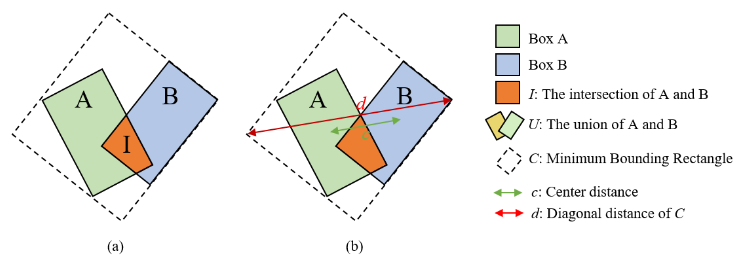
\includegraphics{images/241209/iou.png}
	\caption{新的相似度函数示意图}
\end{figure}

\begin{tcolorbox}
	\textbf{输入:}
	
		\hspace{8em}检测结果	$ B^d=(x^d, y^d,z^d,l^d,w^d,h^d,{\theta}^d) $
		
		\hspace{8em}已有轨迹	$ B^t=(x^t, y^t,z^t,l^t,w^t,h^t,{\theta}^t) $
	
	\textbf{相似度函数}
	
		\hspace{8em}Ro\_GDIoU = $Ro\_IoU - w_1 \cdot \frac{C-U}{C} - w_2 \cdot \frac{c^2}{d^2}$
		
		\hspace{9.5em}Ro\_IoU = $I/U$
		

\end{tcolorbox}

\begin{table}[htbp]
	\centering
	\caption{Pseudo-code of Ro\_GDIoU Algorithm}
	\begin{tabular}{p{0.9\textwidth}}
		\toprule
		\textbf{Algorithm 1: Ro\_GDIoU伪代码} \\
		\midrule
		\textbf{Input:} \\
		检测框, $B_d = (x_d, y_d, z_d, l_d, w_d, h_d, o_d)$ \\
		轨迹框, $B_t = (x_t, y_t, t, l_t, w_t, h_t, \theta_t)$ \\
		\textbf{Output:} \\
		Ro\_GDIoU \\
		\midrule
		1. 转换到BEV空间$B_{\text{bev}}^d, B_{\text{bev}}^t = F_{\text{global} \rightarrow \text{bev}}(B_d, B_t)$ \\
		2. 计算交集$I = F_{\text{inter}}(B_{\text{bev}}^d, B_{\text{bev}}^t)$ \\
		3. 计算并集$U = F_{\text{union}}(B_{\text{bev}}^d, B_{\text{bev}}^t)$ \\
		4. 计算最小外框矩形$C = F_{\text{rect}}(B_{\text{bev}}^d, B_{\text{bev}}^t)$ \\
		5. 中心点距离$c = F_{\text{dist}}(B_{\text{bev}}^d, B_{\text{bev}}^t)$ \\
		6. 外框对角线$d = F_{\text{dist2}}(B_{\text{bev}}^d, B_{\text{bev}}^t)$ \\
		7. Ro-IoU = I/U \\
		8. Ro\_GDIoU = Ro-IoU - $w_1 \cdot \frac{c-u}{w_2 \cdot d^2}$ \\
		($w_1$ 和 $w_2$代表权重) \\
		\bottomrule
	\end{tabular}
\end{table}

\subsection{二阶段的匹配方法}
本文采用了一种从多角度进行匹配的方法,先从BEV空间进行匹配,再从RV空间进行匹配。

\begin{tcolorbox}
	\textbf{坐标变换:}
	\begin{equation}
		C = R \cdot P + T
	\end{equation}
	\begin{equation}
		P=
		\begin{bmatrix}
			\frac{l}{2} & \frac{l}{2} & \frac{l}{2} & \frac{l}{2} & -\frac{l}{2} & -\frac{l}{2} &
			-\frac{l}{2} & -\frac{l}{2} \\
			\frac{w}{2} & -\frac{w}{2} & -\frac{w}{2} & \frac{w}{2} & \frac{w}{2} & -\frac{w}{2} & -\frac{w}{2} & \frac{w}{2} \\
			\frac{h}{2} & \frac{h}{2} & -\frac{h}{2} & -\frac{h}{2} & \frac{h}{2} & \frac{h}{2} & -\frac{h}{2} & -\frac{h}{2}
		\end{bmatrix}
	\end{equation}
	\begin{equation}R=
		\begin{bmatrix}
			\cos(\theta) & -\sin(\theta) & 0 \\
			\sin(\theta) & \cos(\theta) & 0 \\
			0 & 0 & 1
		\end{bmatrix},\quad T=
		\begin{bmatrix}
			x \\
			y \\
			z
		\end{bmatrix}.
	\end{equation}
	
\end{tcolorbox}

\begin{table}[htbp]
	\centering
	\caption{二阶段匹配算法的伪代码}
	\begin{tabular}{p{0.9\textwidth}}
		\toprule
		\textbf{Input:} Trajectory boxes $T$ at time $T-1$, detection boxes $D$ at time $T$ \\

		\textbf{Output:} Matching indices $M$ \\
		\midrule
		\textbf{First matching: BEV Plane} \\
		\hspace{1em} $T_{\text{bev}}, D_{\text{bev}} = F_{3d \rightarrow \text{bev}}(T, D)$ \\
		\hspace{1em} Compute cost $L_{\text{bev}} = \text{Ro-GDIoU}(D_{\text{bev}}, T_{\text{bev}})$ \\
		\hspace{1em} Matching pairs $M_{\text{bev}} = \text{Hungarian}(L_{\text{bev}}, \text{threshold}_{\text{bev}})$ \\
		\midrule
		\textbf{Second matching: RV Plane} \\
		\hspace{1em} For each $d_{\text{bev}} \in D_{\text{bev}}$: \\
		\hspace{2em} If $d_{\text{bev}} \notin M_{\text{bev}}[0]$: \\
		\hspace{3em} $d_{\text{bev}} \rightarrow D_{\text{res}}$ \\
		\hspace{1em} For each $t_{\text{bev}} \in T_{\text{bev}}$: \\
		\hspace{2em} If $t_{\text{bev}} \notin M_{\text{bev}}[1]$: \\
		\hspace{3em} $t_{\text{bev}} \rightarrow T_{\text{res}}$ \\
		\hspace{1em} Matching pairs $M_{\text{rv}} = \text{Greedy}(L_{\text{rv}}, \text{threshold}_{\text{rv}})$ \\
		\midrule
		Obtain the final matching pairs $M = M_{\text{bev}} \cup M_{\text{rv}}$ \\
		\bottomrule
	\end{tabular}
\end{table}
